% 02.rpc.file.transfer.tex
\documentclass[12pt]{article}

% Packages for enhanced functionality
\usepackage{graphicx}      % For including images
\usepackage{listings}      % For code snippets
\usepackage{color}         % For defining colors
\usepackage{geometry}      % For setting margins
\usepackage{hyperref}      % For hyperlinks
\usepackage{caption}       % For customizing captions
\usepackage{float}         % For controlling figure placement

% Page layout
\geometry{
    a4paper,
    left=25mm,
    right=25mm,
    top=25mm,
    bottom=25mm,
}

% Define colors for code
\definecolor{codegreen}{rgb}{0,0.6,0}
\definecolor{codegray}{rgb}{0.5,0.5,0.5}
\definecolor{codepurple}{rgb}{0.58,0,0.82}
\definecolor{backcolour}{rgb}{0.95,0.95,0.92}

% Code listing settings
\lstdefinestyle{mystyle}{
    backgroundcolor=\color{backcolour},   
    commentstyle=\color{codegreen},
    keywordstyle=\color{magenta},
    numberstyle=\tiny\color{codegray},
    stringstyle=\color{codepurple},
    basicstyle=\ttfamily\footnotesize,
    breakatwhitespace=false,         
    breaklines=true,                 
    captionpos=b,                    
    keepspaces=true,                 
    numbers=left,                    
    numbersep=5pt,                  
    showspaces=false,                
    showstringspaces=false,
    showtabs=false,                  
    tabsize=2
}

\lstset{style=mystyle}

% Title and author
\title{RPC-Based File Transfer System Report}
\author{
    \textbf{Group Members:} \\
    Nguyen Ngoc Nhi \\
    Nguyen Duc Duy \\
    Le Viet Hoang Lam \\
    Vu Hai Thien Long \\
    Luu Linh Ly
}
\date{\today}

\begin{document}

\maketitle

\tableofcontents
\newpage

\section{Introduction}
This report outlines our group's RPC-based file transfer system using XML-RPC. The system enables clients to upload files to a centralized server efficiently. The following sections detail the architectural design, system components, implementation specifics with code snippets, and the division of tasks among group members.

\section{RPC Service Design}
The RPC service is designed to facilitate secure and efficient file uploads from clients to the server. Utilizing XML-RPC, the service defines remote procedures that clients can invoke to perform file transfers, incorporating additional steps for authentication, data validation, and error handling.

\subsection{Service Architecture}
The architecture comprises multiple components that interact to ensure reliable file transfers. The key components include:

\begin{itemize}
    \item \textbf{Client Application}: Initiates file upload requests.
    \item \textbf{XML-RPC Service}: Handles remote procedure calls from clients.
    \item \textbf{Authentication Module}: Verifies client credentials.
    \item \textbf{Data Validation Module}: Ensures the integrity and validity of the uploaded data.
    \item \textbf{Server}: Processes and stores the received files.
    \item \textbf{Logging Module}: Records events and errors for monitoring and debugging.
\end{itemize}

\begin{figure}[H]
    \centering
    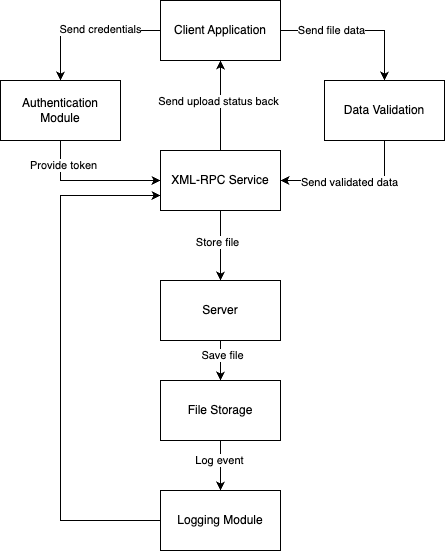
\includegraphics[width=\linewidth]{figure1.png}
    \caption{Detailed RPC Service Architecture}
    \label{fig:detailed_rpc_service_architecture}
\end{figure}

\subsection{Figure Explanation}
\autoref{fig:detailed_rpc_service_architecture} illustrates the interaction between the client, RPC service, and server, incorporating additional modules for authentication, data validation, and logging. The client first authenticates with the Authentication Module to obtain a token, which is then used to interact with the XML-RPC Service. Data sent by the client is validated before being processed by the server. All significant events and errors are logged for monitoring purposes.

\section{Implementation of File Transfer}
The file transfer functionality is implemented using Python's built-in `xmlrpc` libraries. Below are key parts of the implementation for both the server and client, including enhanced error handling and logging.

\subsection{Server Implementation}

\begin{lstlisting}[language=Python, caption={Server-side Implementation}, label={lst:server_code}]
# server.py
from xmlrpc.server import SimpleXMLRPCServer, SimpleXMLRPCRequestHandler
import os
import logging

# Configure logging
logging.basicConfig(filename='server.log', level=logging.INFO,
                    format='%(asctime)s - %(levelname)s - %(message)s')

class RequestHandler(SimpleXMLRPCRequestHandler):
    rpc_paths = ('/RPC2',)

def run_server(host='127.0.0.1', port=8000):
    with SimpleXMLRPCServer((host, port), requestHandler=RequestHandler, allow_none=True) as server:
        server.register_introspection_functions()

        def upload_file(filename, data):
            """
            Receives a file from the client and saves it to the 'received_files' directory.
            
            :param filename: Name of the file to be saved.
            :param data: Binary data of the file.
            :return: Success or failure message.
            """
            try:
                logging.info(f"Received upload request for file: {filename}")
                data_size = len(data.data)
                logging.info(f"Data size received: {data_size} bytes")

                # Ensure the 'received_files' directory exists
                os.makedirs('received_files', exist_ok=True)
                filepath = os.path.join('received_files', filename)

                # Write binary data to the file
                with open(filepath, 'wb') as f:
                    f.write(data.data)
                logging.info(f"Successfully received and saved file: {filepath}")

                return f"File '{filename}' uploaded successfully."
            except Exception as e:
                logging.error(f"Error receiving file '{filename}': {e}")
                return f"Failed to upload file '{filename}'. Error: {str(e)}"

        # Register the upload_file function so clients can call it
        server.register_function(upload_file, 'upload_file')

        logging.info(f"XML-RPC Server listening on {host}:{port}")
        print(f"XML-RPC Server listening on {host}:{port}")
        try:
            server.serve_forever()
        except KeyboardInterrupt:
            logging.info("Shutting down the server.")
            print("\nShutting down the server.")

if __name__ == "__main__":
    run_server()
\end{lstlisting}

\subsection{Client Implementation}

\begin{lstlisting}[language=Python, caption={Client-side Implementation}, label={lst:client_code}]
# client.py
import xmlrpc.client
import os
import logging

# Configure logging
logging.basicConfig(filename='client.log', level=logging.INFO,
                    format='%(asctime)s - %(levelname)s - %(message)s')

def send_file(file_path, server_host='127.0.0.1', server_port=8000):
    """
    Sends a file to the XML-RPC server.

    :param file_path: Path to the file to be sent.
    :param server_host: Server's hostname or IP address.
    :param server_port: Server's port number.
    """
    try:
        # Establish connection to the XML-RPC server
        proxy = xmlrpc.client.ServerProxy(f'http://{server_host}:{server_port}/RPC2')
        logging.info(f"Connected to XML-RPC Server at {server_host}:{server_port}")
        print(f"Connected to XML-RPC Server at {server_host}:{server_port}")

        # Verify that the file exists
        if not os.path.isfile(file_path):
            logging.error(f"File does not exist: {file_path}")
            print(f"Error: File does not exist - {file_path}")
            return

        # Read the file in binary mode
        with open(file_path, 'rb') as f:
            file_data = f.read()
        data_size = len(file_data)
        logging.info(f"Read {data_size} bytes from file '{file_path}'")
        print(f"Read {data_size} bytes from file '{file_path}'")

        filename = os.path.basename(file_path)
        logging.info(f"Uploading file: {filename}")
        print(f"Uploading file: {filename}")

        # Create a Binary object to send binary data
        binary_data = xmlrpc.client.Binary(file_data)
        logging.info(f"Binary data size to send: {len(binary_data.data)} bytes")
        print(f"Binary data size to send: {len(binary_data.data)} bytes")

        # Call the remote method 'upload_file'
        response = proxy.upload_file(filename, binary_data)
        logging.info(f"Server response: {response}")
        print(f"Server response: {response}")

    except xmlrpc.client.ProtocolError as err:
        logging.error(f"Protocol error: {err.errcode} - {err.errmsg}")
        print(f"Protocol error: {err.errcode} - {err.errmsg}")
    except xmlrpc.client.Fault as fault:
        logging.error(f"XML-RPC Fault: {fault.faultString}")
        print(f"XML-RPC Fault: {fault.faultString}")
    except ConnectionRefusedError:
        logging.error(f"Could not connect to server at {server_host}:{server_port}")
        print(f"Could not connect to server at {server_host}:{server_port}")
    except Exception as e:
        logging.error(f"An unexpected error occurred: {e}")
        print(f"An unexpected error occurred: {e}")

if __name__ == "__main__":
    file_path = input("Enter the path to the file you want to send: ").strip()
    send_file(file_path)
\end{lstlisting}



\section{Implementation of File Transfer Diagram}
To provide a more detailed visualization of the file transfer process, the following diagram outlines each step involved in uploading a file from the client to the server, including authentication, data validation, and logging.

\begin{figure}[H]
    \centering
    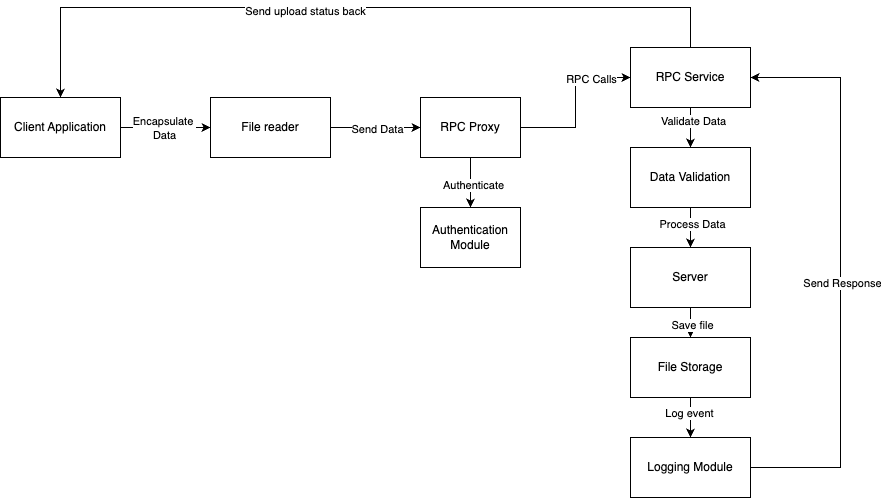
\includegraphics[width=\linewidth]{figure2.png}
    \caption{Implementation of File Transfer Diagram}
    \label{fig:implementation_file_transfer}
\end{figure}

\subsection{Figure Explanation}
\autoref{fig:implementation_file_transfer} provides a step-by-step view of the file transfer process:

\begin{enumerate}
    \item **Read File**: The client reads a file from its local filesystem.
    \item **Encapsulate Data**: The file data is wrapped into a binary format suitable for transmission.
    \item **Send Encapsulated Data**: The wrapped data is sent to the RPC Proxy.
    \item **Authenticate**: The RPC Proxy sends authentication credentials to the Authentication Module.
    \item **Provide Token**: Upon successful authentication, the Authentication Module returns a token to the RPC Service.
    \item **RPC Calls**: The RPC Proxy handles remote procedure calls from the client.
    \item **Validate Data**: The RPC Service sends the file data to the Data Validation Module for integrity checks.
    \item **Process Data**: The Data Validation Module forwards validated data to the Server for processing.
    \item **Store File**: The RPC Service instructs the Server to store the received file.
    \item **Save File**: The Server saves the file to the File Storage module.
    \item **Log Activity**: The Server logs the file transfer event in the Logging Module.
    \item **Send Status**: The Response Handler sends a status message back to the client regarding the upload.
\end{enumerate}

This detailed flow ensures that each step is validated and logged, enhancing the reliability and maintainability of the system.

\section{Team Responsibilities}
Our group of five members collaborated efficiently by dividing the tasks based on individual strengths and project requirements. Below is the distribution of responsibilities:

\begin{itemize}
    \item \textbf{Nguyen Ngoc Nhi}:
    \begin{itemize}
        \item Designed the overall RPC service architecture.
        \item Created detailed system diagrams using TikZ.
    \end{itemize}
    
    \item \textbf{Nguyen Duc Duy}:
    \begin{itemize}
        \item Implemented the server-side code (`server.py`).
        \item Managed the file storage system and server configurations.
    \end{itemize}
    
    \item \textbf{Le Viet Hoang Lam}:
    \begin{itemize}
        \item Developed the client-side code (`client.py`).
        \item Handled data transmission and client error handling.
    \end{itemize}
    
    \item \textbf{Vu Hai Thien Long}:
    \begin{itemize}
        \item Assisted in designing system diagrams.
        \item Conducted testing and debugging of the file transfer process.
    \end{itemize}
    
    \item \textbf{Luu Linh Ly}:
    \begin{itemize}
        \item Compiled and wrote the project report.
        \item Coordinated team meetings and ensured timely completion of tasks.
    \end{itemize}
\end{itemize}

\section{Conclusion}
Our RPC-based file transfer system successfully enables clients to upload files to a server using XML-RPC. Through careful architectural design, modular implementation, and effective teamwork, the system ensures secure, reliable, and efficient file transfers. Future enhancements could include implementing SSL/TLS for secure communications, supporting larger files through chunked transfers, and adding functionality for file downloads.

\end{document}
